\RequirePackage{luatex85}
\documentclass[tikz, border=10pt]{standalone}
\usetikzlibrary{shapes.geometric, arrows}
\usetikzlibrary{positioning}
\usepackage{physics}

\tikzstyle{selection} = [rectangle, rounded corners, minimum width=3cm, minimum height=1.5cm, text centered, text width=4.0cm, draw=black, fill=white]

\tikzstyle{arrow} = [thick,->,>=stealth]

\begin{document}

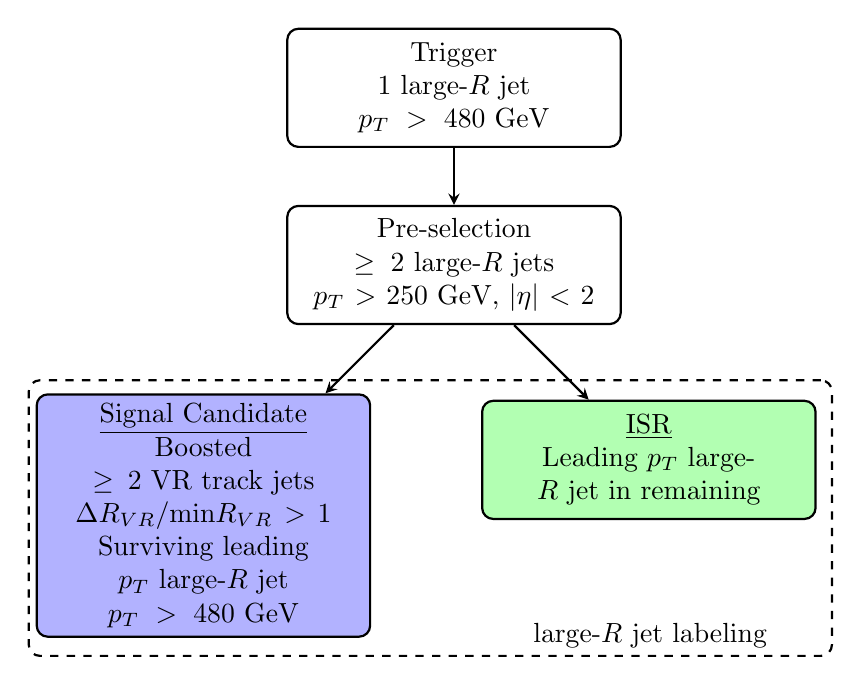
\begin{tikzpicture}[thick, node distance=2.25cm]
 \node (trigger) [selection] {Trigger\\1 large-$R$ jet\\$p_{T} > 480~\textrm{GeV}$};
 \node (pre) [selection, below of=trigger] {Pre-selection\\$\geq 2$ large-$R$ jets\\$p_{T} > 250~\textrm{GeV}$, $\abs{\eta} < 2$};
 \node (signal) [selection, below left of=pre, node distance=4.5cm, fill=blue!30] {\underline{Signal Candidate}\\Boosted\\$\geq2$ VR track jets\\ $\Delta R_{VR}/\mathrm{min} R_{VR} > 1$\\Surviving leading\\ $p_{T}$ large-$R$ jet\\$p_T > 480~\textrm{GeV}$};
 \node (ISR) [selection, below right of=pre, node distance=3.5cm, fill=green!30] {\underline{ISR}\\Leading $p_{T}$ large-$R$ jet in remaining};

 \draw [arrow] (trigger) -- (pre);
 \draw [arrow] (pre) -- (signal);
 \draw [arrow] (pre) -- (ISR);
 \node (jet_box) [selection, dashed, minimum width=10.2cm, minimum height=3.5cm, fill=none, below] at (-0.3,-3.7) {};
 \node (jet_box_text) [below right of=jet_box, xshift=1.2cm, yshift=0.1cm] {large-$R$ jet labeling};
\end{tikzpicture}
\end{document}
